\subsection{Heurística constructiva de cluster-first, route-second, clusterizando con algoritmo de K-means}
\subsubsection{El algoritmo}\label{kmeans-el-algoritmo}
\paragraph{}
Resolver de forma heurística el problema de CVRP mediante un algoritmo cluster-first, route-second se divide en dos partes : \textbf{1.} la clusterización y \textbf{2.} la búsqueda de un camino mínimo. Como mencionamos en \ref{subsection:sweep} hay distintas maneras de separar en clusters y de luego buscar esas posibles rutas. Una fue la técnica de \textit{Sweeping}. La que desarrollaremos a continuación, clusterizará mediante el algoritmo de \textit{k-means} y resolverá los TSP restantes mediante \textit{Nearest Neighbour}.
\textbf{K-means} consiste en asignar cada punto al cluster cuyo centro, que llamaremos $centroid$, se encuentra más cerca. Definiremos el centroid de cada cluster k como la media entre todos los puntos que pertenecen a dicha partición. Veamos los pasos en detalle:

\begin{description}
	\item[Paso 1.] Elegimos $k$ cantidad de clusters. Seleccionamos un valor aproximado al posible total de camiones que utilizará nuestro algoritmo. Por eso, decidimos elegir el promedio de los productos que llevará cada camión (es decir, el promedio de demanda solicitada por viaje). Decimos que es aproximado ya que en nuestra implementación permitimos que se agreguen clusters de ser necesario.
	\item[Paso 2.] Seleccionamos $k$ puntos como centroids de los $k$ clusters. Como los puntos de la entrada no tienen un orden particular, elegimos los $k$ primeros. Otra opción era elegirlos random, los de mayor/menor demanda, etc.
	\item[Paso 3.] Asignamos cada punto al centroid más cercano. Para ello ordenamos los clusters según distancia al punto en cuestión. Luego, desde el más cercano al más lejano, buscamos el primero cuya capacidad restante mas la demanda del cliente no supere la capacidad total. Si no queda espacio en ningún camión, creamos nuevo cluster con centroid en el mismo punto.
	\item[Paso 4.] Después de recorrer los vértices, calculamos los nuevos centroids de cada cluster.
	\item[Paso 5.] Repetimos el procedimiento hasta que los puntos dejen de cambiar de cluster: no haya más asignaciones en el paso 4.
\end{description}
Sean $(x_{1}, y_{1}), (x_{2}, y_{2})...(x_{m_{j}}, y_{m_{j}})$ los $m_{j}$ puntos pertenecientes al cluster $j$, definiremos su centroid como $c_{j}=(X_{j}, Y_{j})$ donde: \\
$$ x_{j} = \sum_{i=1}^{m_{j}} x_{i}/m_{j}$$
$$ y_{j} = \sum_{i=1}^{m_{j}} y_{i}/m_{j}$$
$$ c_{j}=(x_{j}, y_{j}) $$
\paragraph{} 
Es decir, el promedio en cada coordenada. Cabe resaltar además que es importante que los clusters no compartan nodos entre sí, no puede haber al mismo tiempo dos camiones que vayan al mismo punto. Por lo tanto, se cumple que la cantidad total de puntos $n$ es $\sum_{i=1}^{k} m_{j}$. Además, como solo se agregan clientes a clusters donde es posible satisfacer su demanda, se verifica que para todo cluster $j$ $\sum_{i=1}^{m_{j}} demanda(cliente_{i}) <= C$.
\\
\par Finalmente, cuando terminamos de clusterizar procedemos al armado de rutas.
\begin{enumerate}
	\item Agregamos cada punto a su cluster efectivo.
	\item Si quedaron clusters vacios, los eliminamos.
	\item Aplicamos la heurística de \textit{Nearest Neighbour} para cada cluster.
	\item Retornamos el conjunto de camiones con sus respectivas rutas.
\end{enumerate}

\subsubsection{Pseudo-código}

\begin{algorithm}[H]
	\caption{\Comment $\mathcal{O}(cant\_it * n*k*\log(k)+n ^2*log(n)) = \mathcal{O}(n^2*log(n))$}
	\begin{algorithmic}[1]
		\Function{resolverCVRP}{Punto $deposito$, Conjunto de puntos $puntos$, Entero $capacidad$}
		\State $n \gets |puntos|$
		\State $k \gets \textbf{calcularK}(puntos, capacidad)$ \Comment $\mathcal{O}(n)$
		\Statex
		\State \textbf{Vector de Enteros} $en\_que\_cluster\mathcal{}(n, ninguno)$
		\State \textbf{Vector de Puntos} $k\_clusters$
		\State \textbf{InicializarClusters}$(puntos, k\_clusters, en\_que\_cluster, capacidad)$  \Comment $\mathcal{O}(k)$
		\Statex
		\While{sigue cambiando}
		\For{$i$ desde $0$ hasta $n-1$}
		\State $ultimo\_cluster \gets en\_que\_cluster[i]$
		\State $cluster \gets $ \textbf{centroidMasCercano}$(k\_clusters, puntos[i], ultimo\_cluster)$ \Comment $\mathcal{O}(k*\log(k))$
		\If{$ultimo\_cluster \neq cluster$}
		\State $en\_que\_cluster[i] \gets cluster$
		\State $k\_clusters[cluster].demand \gets k\_clusters[cluster].demand-puntos[i].demand$
		\If{$ultimo\_cluster \neq ninguno$}
		\State $k\_clusters[ultimo\_cluster].demand \gets k\_clusters[ultimo\_cluster].demand + puntos[i].demand$
		\EndIf
		\EndIf
		\EndFor
		\For{$i$ desde $0$ hasta $k-1$}
		\State \textbf{Punto } $nuevo\_centroid \gets $ \textbf{calcularCentroid}$(en\_que\_cluster, k\_clusters[i].demand, i, puntos)$ \Comment $\mathcal{O}(n)$
		\If{$nuevo\_centroid \neq k\_clusters[i]$}
		\State $k\_clusters[i] \gets nuevo\_centroid$
		\EndIf
		\EndFor
		\EndWhile
		\Statex
		\State \textbf{Lista de clusters} $clusters \gets $ \textbf{ConstruirClusters}$(puntos, en\_que\_cluster)$ \Comment $\mathcal{O}(n)$
		\State \textbf{Rutas} $rutas \gets$ \textbf{ConstruirRutasAPartirDeClusters}$(clusters, deposito, capacidad)$ \Comment $\mathcal{O}(n^2*log(n))$
		\Statex
		\State \Return $rutas$
		\EndFunction
	\end{algorithmic}
\end{algorithm}

\paragraph{Inicialización}

\begin{itemize}
	\item Inicializamos $en\_que\_cluster$ con el define $ninguno$: para cada punto $i$, $en\_que\_cluster[i]$ representará el cluster al que pertenece $i$. 
	\item Calculamos la cantidad de clusters según \ref{calcular-k}. Como mencionamos anteriormente, dependerá de la capacidad de los camiones y de la demanda de los clientes.
	\item Elegimos los primeros $k$ puntos que funcionarán como nuestros primeros centroids según \ref{inicializar-clusters}. Cada centroid tendrá la misma estructura que los puntos: tendrá su componente y, su componente x y un entero que almacenará la capacidad que le queda al camión que visitará todos los puntos pertenecientes a dicho cluster.
\end{itemize}

\begin{algorithm}[H]
	\caption{\Comment $\mathcal{O}(n)$}
	\label{calcular-k}
	\begin{algorithmic}[1]
		\Function{calcularK}{Vector de Puntos $puntos$, Entero $capacidad$}
		\State \textbf{Real } $nuevo\_k \gets 0$
		\For{cada $p$ en $puntos$} \Comment $\mathcal{O}(n)$
		\State $nuevo\_k \gets nuevo\_k + p.demand$
		\EndFor
		\State $nuevo\_k \gets nuevo\_k/capacidad$ 
		\State \Return \textbf{ceil}$(nuevo\_k)$
		\EndFunction
	\end{algorithmic}
\end{algorithm}

\begin{algorithm}[H]
	\caption{\Comment $\mathcal{O}(k)$}
	\label{inicializar-clusters}
	\begin{algorithmic}[1]
		\Function{inicializarClusters}{Vector de Puntos $puntos$, Vector de Puntos $k\_clusters$, Vector de Enteros $en\_que\_cluster$, Entero $capacidad$}
		\For{$i$ desde $0$ hasta $k-1$} \Comment $\mathcal{O}(k)$
		\State $k\_clusters$\textbf{.agregarAtras}$(Punto(puntos[i].x, puntos[i].y, capacidad - puntos[i].demand))$
		\State $en\_que\_cluster[i] \gets |k\_clusters|-1$
		\EndFor
		\EndFunction
	\end{algorithmic}
\end{algorithm}


\paragraph{Ciclo}
\paragraph{}
El ciclo iterará hasta que los puntos dejen de cambiar de cluster o hasta que se llegue a una cantidad constante elegida de iteraciones (lo explicaremos en la siguiente sección).\hspace{0pt} \\
\indent \textbf{Actualización de puntos:} por cada punto calcularemos el centroid más cercano. Si no pertenece al mismo cluster al que pertenecía antes, actualizamos $en\_que\_camion$ con el nuevo cluster. Además, hay que restarle a la capacidad restante del nuevo la demanda del cliente (es suficiente porque se chequeó en \textbf{centroidMasCercano}) y al viejo, devolverle la capacidad que ya no se usa. Cabe resaltar que en la primera iteración del ciclo habrá puntos que no pertenezcan a ningún cluster y por ende, esa demanda no deberá ser devuelta a ningún camión.\hspace{0pt} \\
\indent \textbf{Actualización de centroids:} Por cada cluster $i$ entre los $k$, como se actualizó la pertenencia de los puntos en los clusters, se debe actualizar el centro que lo representa.  \textbf{calcularCentroid} devolverá el nuevo punto promedio del cluster o en caso de que no haya puntos, un punto inválido. La idea es que $Punto\_Invalido$ tenga capacidad negativa para que no se le pueda volver a asignar a ese cluster ningún punto en el primer for.

\paragraph{Auxiliar: centroid más cercano}
\paragraph{} El algoritmo \ref{centroid-mas-cercano} buscará el cluster cuyo centroid se encuentre más cerca al punto pasado por parámetro. Para esto, ordenamos una copia del vector de clusters por distancia a este de forma creciente. Como hay $k$ centroids, esto pertenece a $\mathcal{O}(k*\log(k))$.  Al iterar tendremos tres casos:
\begin{enumerate}
	\item El punto no estaba en ningún cluster: el primer cluster que encuentre que tenga capacidad suficiente para la demanda del cliente, será el resultado.
	\item El punto no cambia de cluster: todos los que encontré antes de $k\_clusters[ultimo\_cluster]$ no tienen capacidad suficiente. Como el cliente ya era visitado por ese camión, la capacidad no debe ser chequeada.
	\item El punto cambia de cluster: o bien encontré uno con capacidad suficiente o tengo que agregar uno nuevo.
\end{enumerate} 
\paragraph{}Como el ciclo termina con $i$ = $indice\_del\_cluster$+1, si no creé uno nuevo, devuelvo la posición en el vector sin ordenar del centroid $i-1$. Como eso significa recorrer $k\_clusters$, es $\mathcal{O}(k)$. Por último, en el caso en que se cree uno nuevo, se agrega un cluster con centroid en el $punto$ y se devuelve su posición.
\begin{algorithm}[H]
	\caption{\Comment $\mathcal{O}(k*\log(k))$}
	\label{centroid-mas-cercano}
	\begin{algorithmic}[1]
		\Function{centroidMasCercano}{Vector de Puntos $k\_clusters$, Punto $punto$, Entero $ultimo\_cluster$}
		\State \textbf{Punto } $viejo\_centroid \gets k\_clusters[0]$
		\If{$ultimo\_cluster \neq ninguno$}
		\State $viejo\_centroid \gets k\_clusters[ultimo\_cluster]$
		\EndIf 
		\State \textbf{Entero } $i \gets 0$
		\State \textbf{Bool } $termine \gets false$
		\State \textbf{ordenarPorDistancia}$(copia\_de\_clusters(k\_clusters), punto)$ \Comment $\mathcal{O}(k*\log(k))$
		\Statex
		\While{$i < k$ $\land$  $\neg termine$} \Comment $\mathcal{O}(k)$
		\If{$ultimo\_cluster = ninguno \vee viejo\_centroid \neq copia\_de\_clusters[i]$}
		\State \textbf{Entero } $capacidad\_restante \gets copia\_de\_clusters[i].demand$ 
		\If{$capacidad\_restante >= punto.demand$}
		\State $termine \gets true$
		\EndIf
		\Else
		\State $termine \gets true$
		\EndIf
		\State $i \gets i+1$
		\EndWhile
		\Statex
		\If{$\neg termine$}
		\State $k\_clusters$\textbf{.agregarAtras}$(punto)$
		\State $k \gets k+1$
		\State \Return $k-1$
		\EndIf
		\State \Return \textbf{indiceEnVec}$(k\_clusters, copia\_de\_clusters[i-1])$  \Comment $\mathcal{O}(k)$
		\EndFunction
	\end{algorithmic}
\end{algorithm}

\paragraph{Calcular centroid}
\paragraph{} El algoritmo \ref{calcular-centroid} calcula el promedio en cada componente de todos los puntos del cluster pasado por parámetro. Si está vacio, devuelve $Punto\_invalido$. Como recorre todos los puntos y chequea si pertenecen a dicho cluster, pertenece a $\mathcal{O}(n)$.
\paragraph{Armado de rutas}
\paragraph{} Al igual que para la otra heurística cluster-first, route-second crearemos los clusters efectivos y resolveremos los TSP restantes mediante \textit{Nearest Neighbour}.  Para construirlos, utilizamos \ref{construir-clusters} que recorre $en\_que\_cluster$ y agregara los respectivos puntos a cada Cluster (renombre de vector de puntos). Un agregado de la implementación fue antes de armar las rutas eliminar los clusters vacios, lo cual no agrega complejidad ya que recorrer y borrar pertenece a $\mathcal{O}(k)$. Por último, resolvemos los TSP mediante \ref{sweep-build-routes}, de complejidad $\mathcal{O}(n^2*log(n))$.
\begin{algorithm}[H]
	\caption{\Comment $\mathcal{O}(n)$}
	\label{calcular-centroid}
	\begin{algorithmic}[1]
		\Function{calcularCentroid}{Vector de Enteros $en\_que\_cluster$, Entero $demanda$, Entero $cluster$, Vector de Puntos $puntos$}
		\State \textbf{Real } $mean\_x \gets 0$
		\State \textbf{Real } $mean\_y \gets 0$
		\State \textbf{Entero } $cant \gets 0$
		\For{$i$ desde $0$ hasta $n-1$} \Comment $\mathcal{O}(n)$
		\If{$en\_que\_cluster[i]=cluster$}
		\State $mean\_x \gets mean\_x + puntos[i].x$
		\State $mean\_y \gets mean\_y + puntos[i].y$
		\State $cant \gets cant+1$
		\EndIf
		\EndFor
		\If{$cant=0$}
		\State \Return $Punto\_Invalido$
		\EndIf
		\State \Return \textbf{Punto}$(mean\_x/cant, mean\_y/cant)$
		\EndFunction
	\end{algorithmic}
\end{algorithm}

\begin{algorithm}[H]
	\caption{\Comment $\mathcal{O}(n)$}
	\label{construir-clusters}
	\begin{algorithmic}[1]
		\Function{ConstruirClusters}{Vector de puntos $puntos$, Vector de Enteros $en\_que\_cluster$}
		\State \textbf{Lista de Cluster} $clusters$(k, $\varnothing$)
		\Statex
		\For{$i$ desde $0$ hasta $n-1$}\Comment $\mathcal{O}(n)$
		\State $clusters[en\_que\_cluster[i]]$\textbf{.agregarAtras}$(puntos[i])$
		\EndFor
		\Statex
		\State \Return $clusters$
		\EndFunction
	\end{algorithmic}
\end{algorithm}

\subsubsection{Análisis de complejidad}
\paragraph{Complejidad espacial} \hspace{0cm}\\
\\
Contamos con varios vectores de tamaño $n$ y de tamaño $k$. Como $k$ está acotado por $n$, la complejidad espacial pertenece a $\mathcal{O}(n)$.
\paragraph{Complejidad temporal}
\begin{itemize}
	\item Inicialización de vectores en $\mathcal{O}(n)$.
	\item \textbf{calcularK} pertenece a $\mathcal{O}(n)$.
	\item Dentro del ciclo, se efectua para cada punto \textbf{centroidMasCercano}, que es $\mathcal{O}(k*log(k))$. Por lo tanto, el primer for tiene una complejidad de $\mathcal{O}(n*k*log(k))$
	\item El segundo for itera $k$ veces mientras que \textbf{calcularCentroid} tiene de complejidad $\mathcal{O}(n)$. Todo junto es $\mathcal{O}(k*n)$, absorvido por el primer for.
	\item El armado de clusters pertenece a $\mathcal{O}(n)$.
	\item El de rutas, es $\mathcal{O}(n^2*log(n))$.
\end{itemize}
\paragraph{}El ciclo iterará hasta que los puntos dejen de cambiar de cluster. Por lo tanto, la complejidad queda:
$$\mathcal{O}(cant\_it *n*k*\log(k)+n^2*log(n))$$
\paragraph{}
Sin embargo, como de heurísticas se habla, estamos buscando llegar a una solución aproximada del problema. En consecuencia, decidimos acotar la cantidad de iteraciones que realizará el ciclo. Cuando analicemos como funciona el algoritmo con los data sets provistos, veremos que en general se realizan pocas iteraciones al ciclo por lo que elegimos una cota un poco más grande que el mayor experimentado. 
\paragraph{}
Teniendo esto en cuenta y como $k$ está acotado por $n$, la complejidad del algoritmo es:
$$\mathcal{O}(cant\_it *n*k*\log(k)+n^2*log(n)) = \mathcal{O}(n*k*\log(k)+n^2*log(n))= \mathcal{O}(n^2*log(n))$$
\subsubsection{Instancias con soluciones no óptimas}
\subsubsubsection{Ver más allá}
Por la naturaleza de la heurística y como veremos en la experimentación, $Savings$ suele dar una solución eficiente. Sin embargo, sigue siendo una heurística y no es seguro que de valores cercanos a la solución óptima. Como ya mencionamos, no es fácil resolver este problema exactamente por lo que una aproximación a la solución es una buena idea: savings podría dar una muy buena solución inicial y a partir de ella, ser mejorada con técnicas computacionales o incluso por humanos. Es interesante esta idea, ya que en ciertos casos a veces tendemos a imaginar que el algoritmo debería ver ``mas allá'', al igual que el ojo humano. Por eso, una persona podría encontrar una mejora en los caminos propuestos por una heurística con facilidad.
\par 
El concepto de ``no ver a futuro'' es lo que hace que savings pueda tener malos casos. Recorre las posibles conexiones de nodos que producen la mayor ganancia en distancia pero eligiéndolas siempre que puede. Es decir, si la ruta es factible y el camión que la recorre tiene la capacidad suficiente, el respectivo saving es elegido, las rutas mergeadas, los nodos conectados. En consecuencia, cada opción tomada restringirá a las siguientes. El caso obvio de esto son las restricciones de capacidad pero no tenemos que olvidar que para poder usar la conexión de dos nodos ninguno puede ser un nodo interno (en ese caso, ya fue conectado a dos vecinos y como son caminos hamiltonianos, no es posible la unión con un tercero). A partir de esto surge el razonamiento de que ocurriría si se saltea un saving pensando a futuro.  
\par 
Esta es la idea del algorítmo de \textbf{Holmes and Parker}, cuyo principio es permitir la prohibición de conexiones (que aunque tengan valor alto de saving) afecten las posibles conexiones siguientes. De esta forma, se forma un árbol de posibles soluciones con cada decisión tomada y se elige la mejor. Las condición para parar podrían depender de hasta que punto estamos dispuestos a explorar, el tamaño del árbol, etc.
\subsubsubsection{Rutas circulares}
El efecto inmediato de lo mencionado anteriormente es que una conexión no pueda ser deseleccionada. Por lo tanto, sobre todo cuando la capacidad es ajustada, savings suele armar cierto tipo de rutas, periféricas, circulares. 
\par 
Más específicamente, tomamos instancias donde no da una solución óptima y la comparamos con ella.
\begin{figure}[H]
	\centering
	\begin{minipage}{0.35\textwidth}
		\centering
		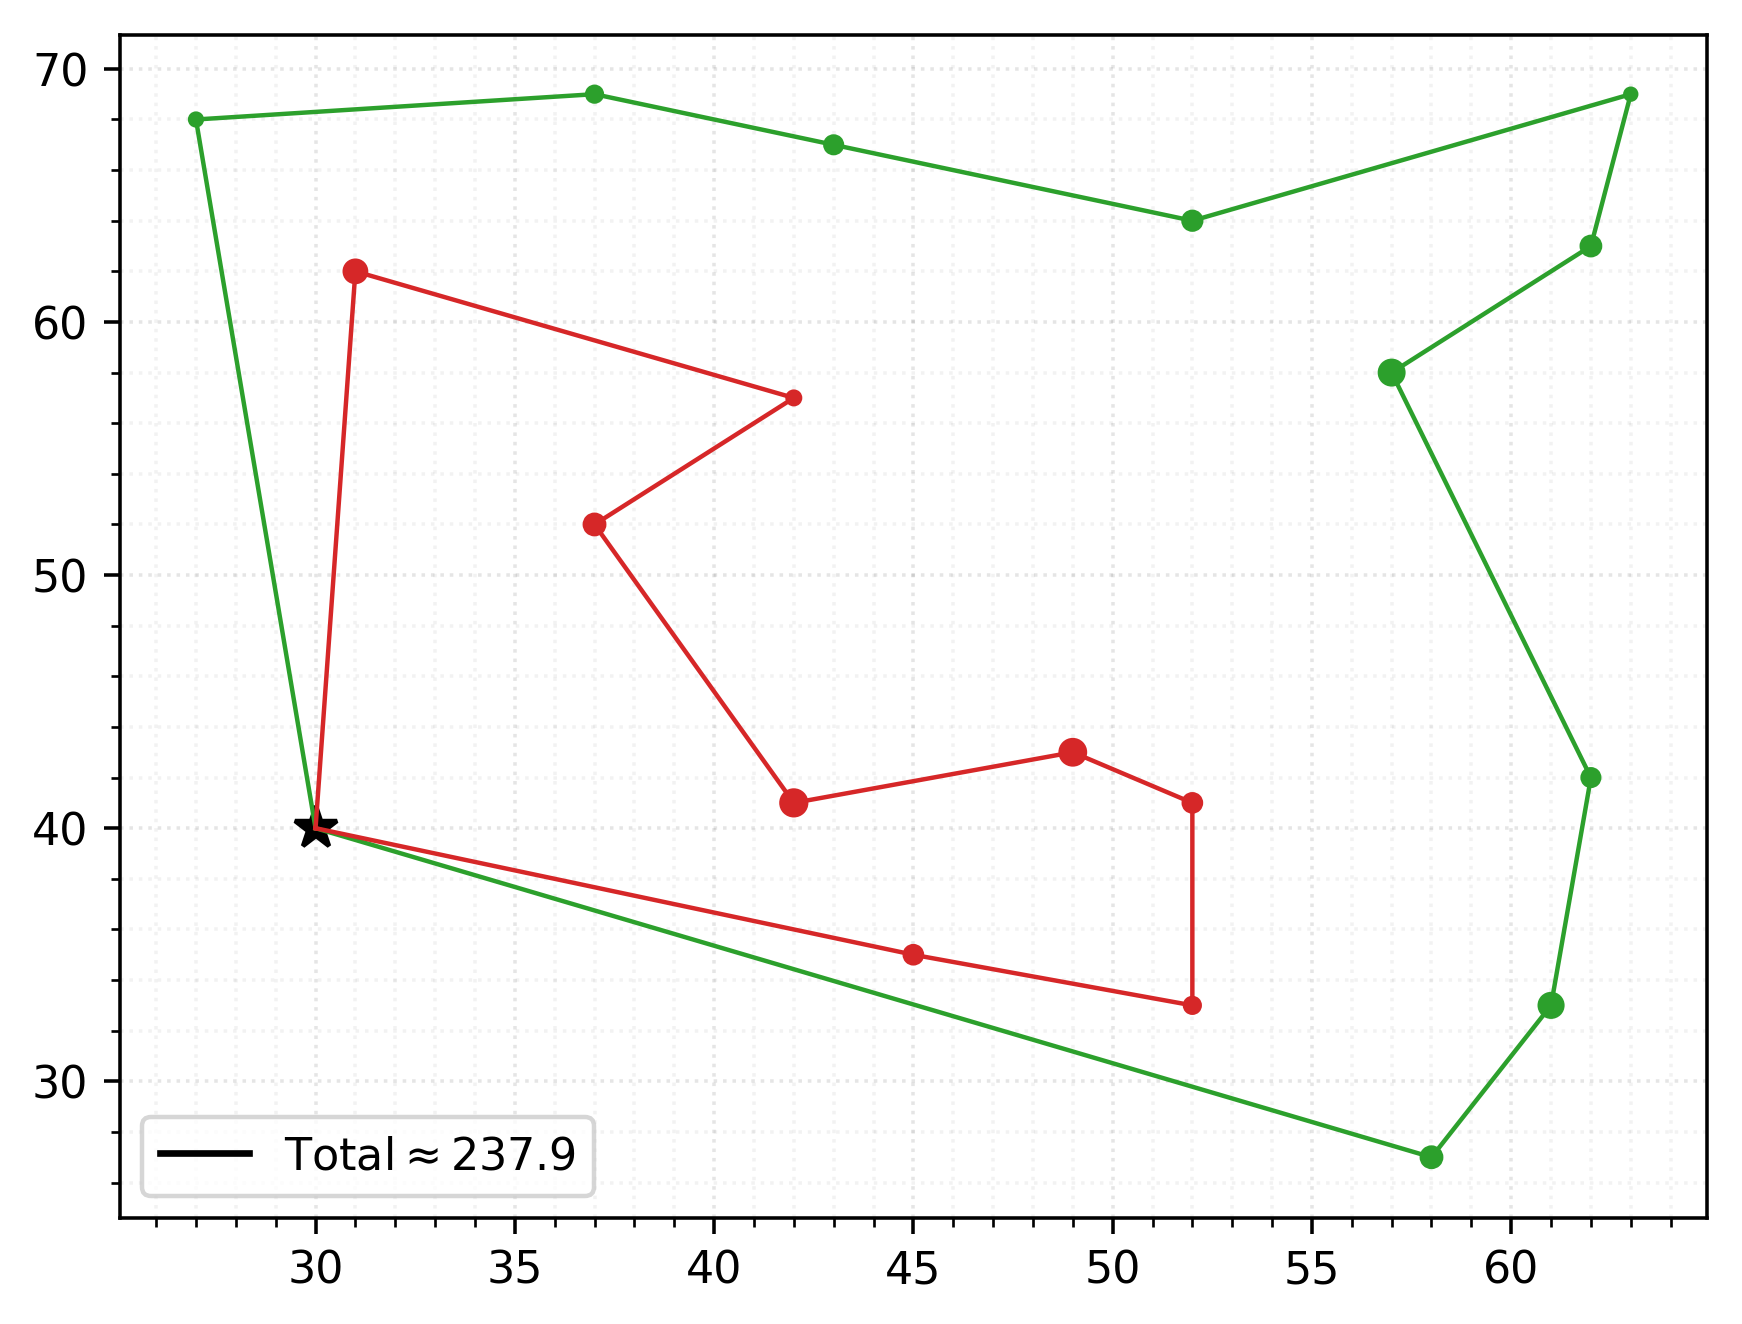
\includegraphics[width=1\textwidth]{images/savings/malosavingchico2}
		\caption{\footnotesize Ruta resultado savings para la instancia \textbf{P-n19-k2}}
		\label{fig:savings-malo-chico2}
	\end{minipage}%
	\hspace{0.03\textwidth}
	\begin{minipage}{0.35\textwidth}
		\centering
		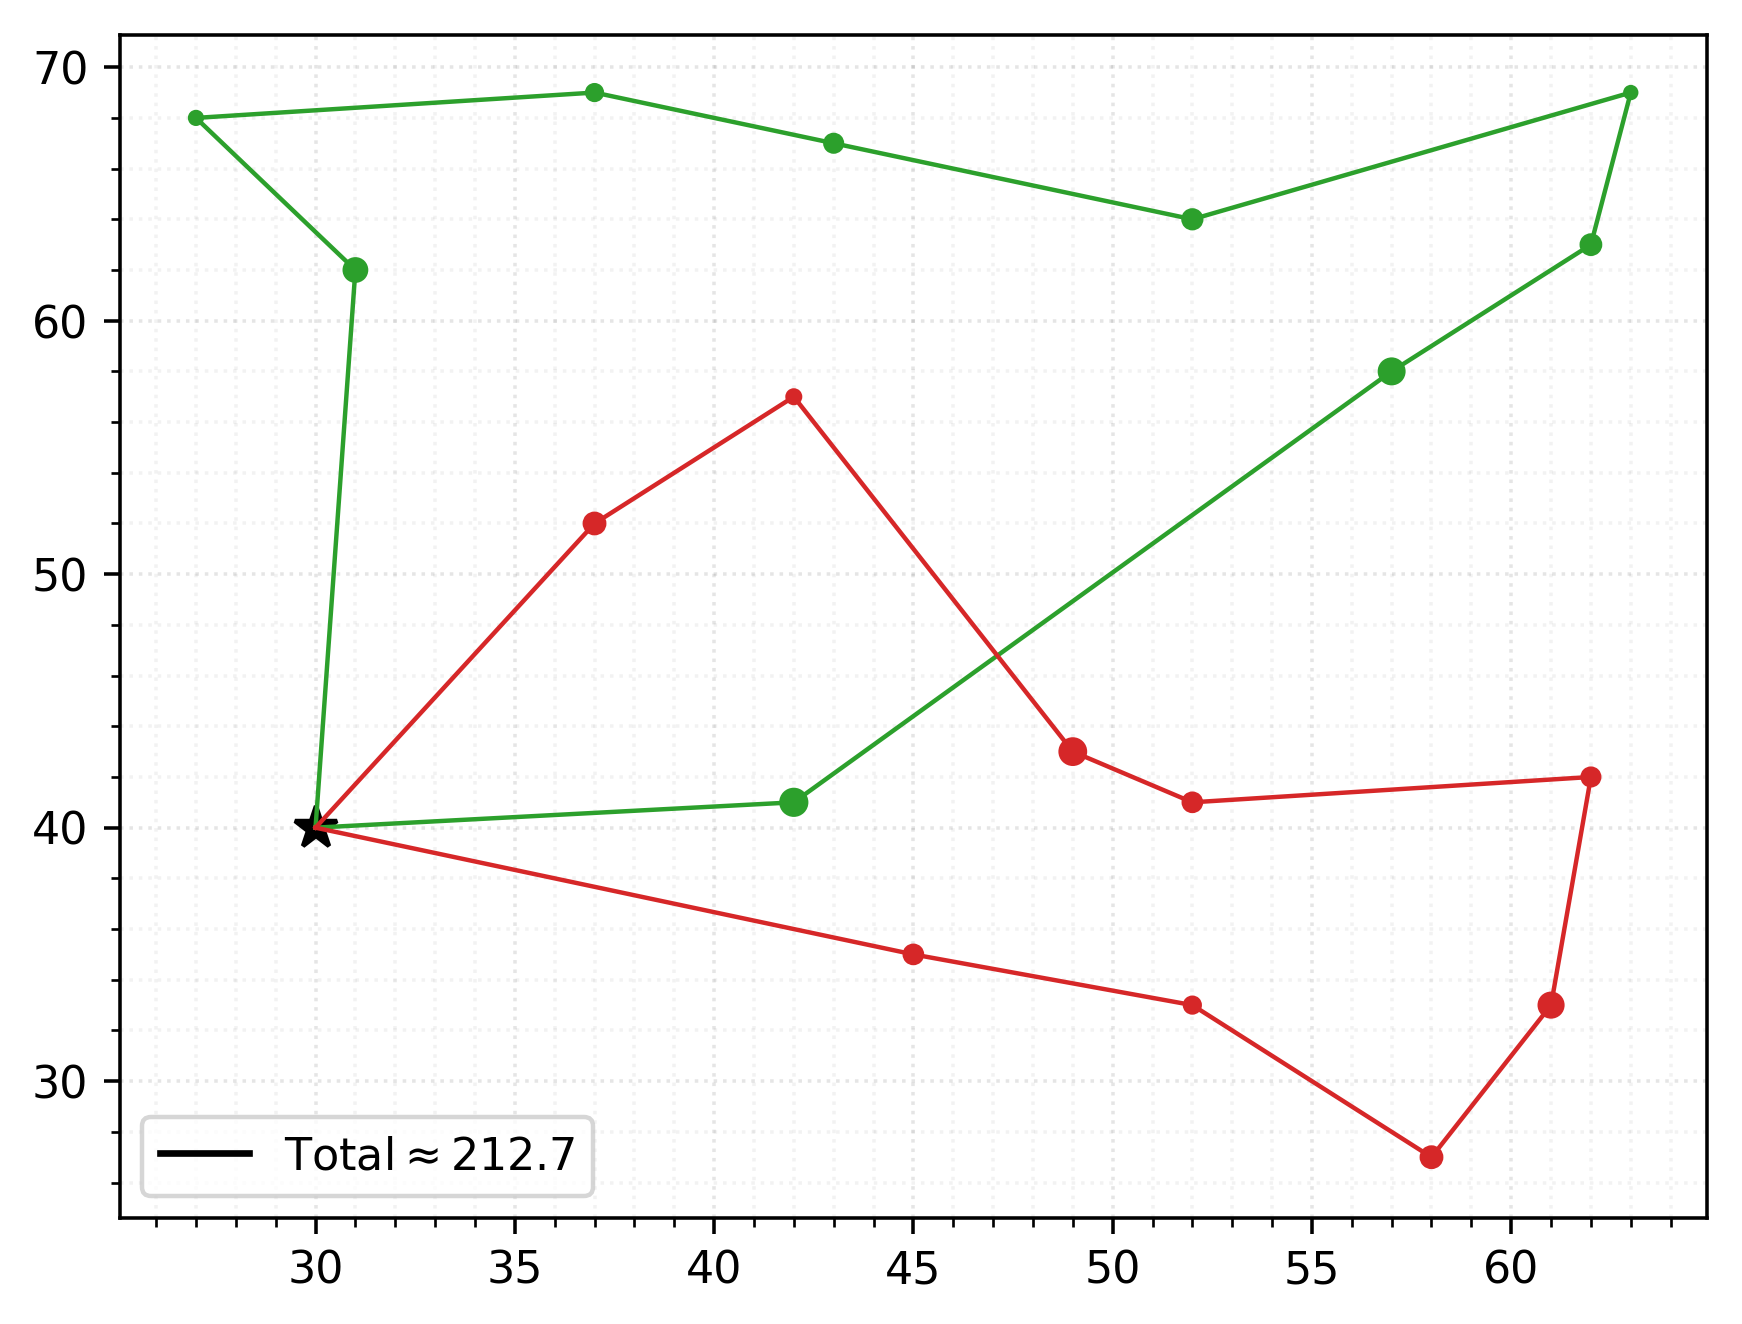
\includegraphics[width=1\textwidth]{images/savings/optimochico2}
		\caption{\footnotesize Ruta óptima para la instancia \textbf{P-n19-k2}}
		\label{fig:savings-optimo-chico2}
	\end{minipage}%
\end{figure}
\begin{figure}[H]
	\centering
	\begin{minipage}{0.35\textwidth}
		\centering
		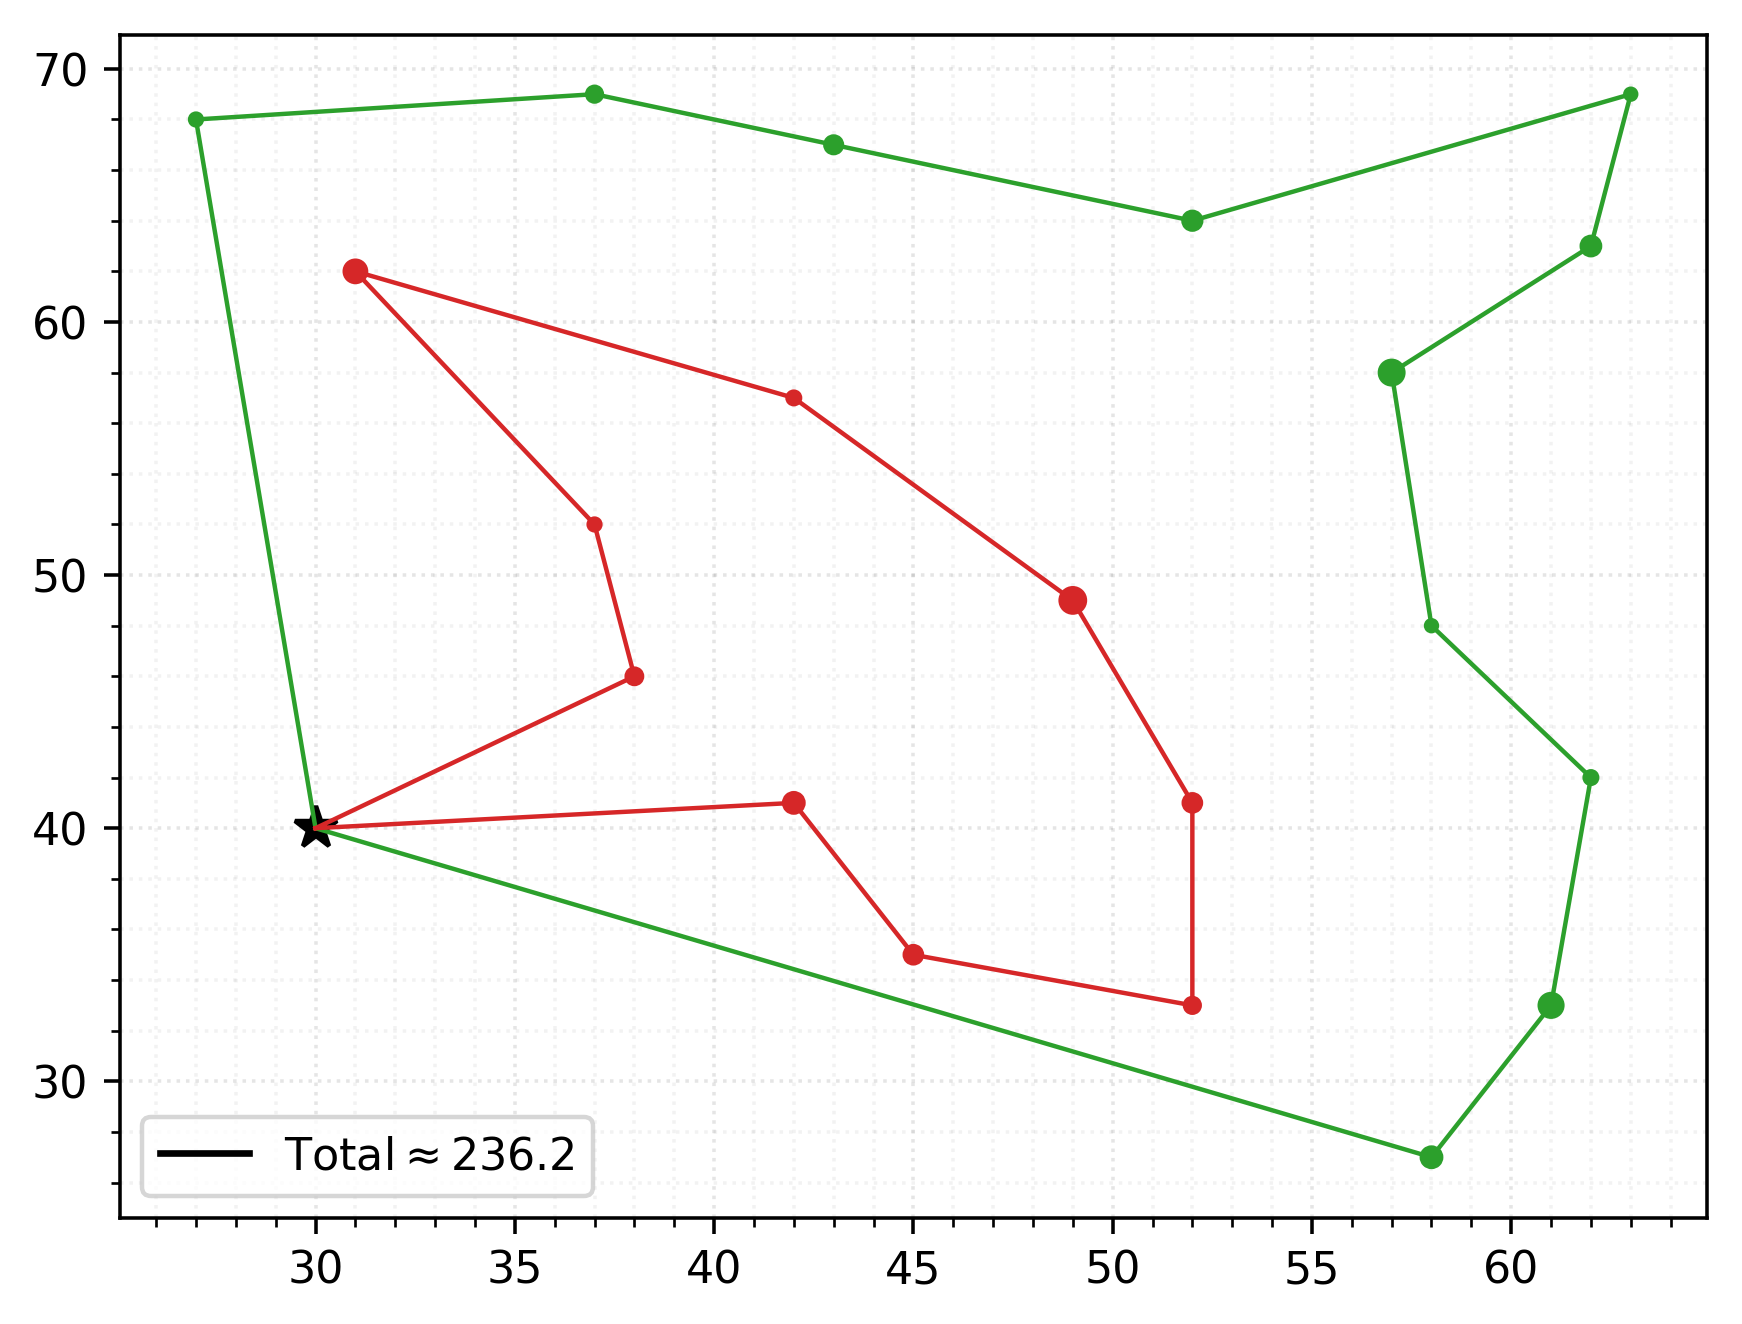
\includegraphics[width=1\textwidth]{images/savings/malosavingchico}
		\caption{\footnotesize Ruta resultado savings para la instancia \textbf{P-n21-k2}}
		\label{fig:savings-malo-chico}
	\end{minipage}%
	\hspace{0.03\textwidth}
	\begin{minipage}{0.35\textwidth}
		\centering
		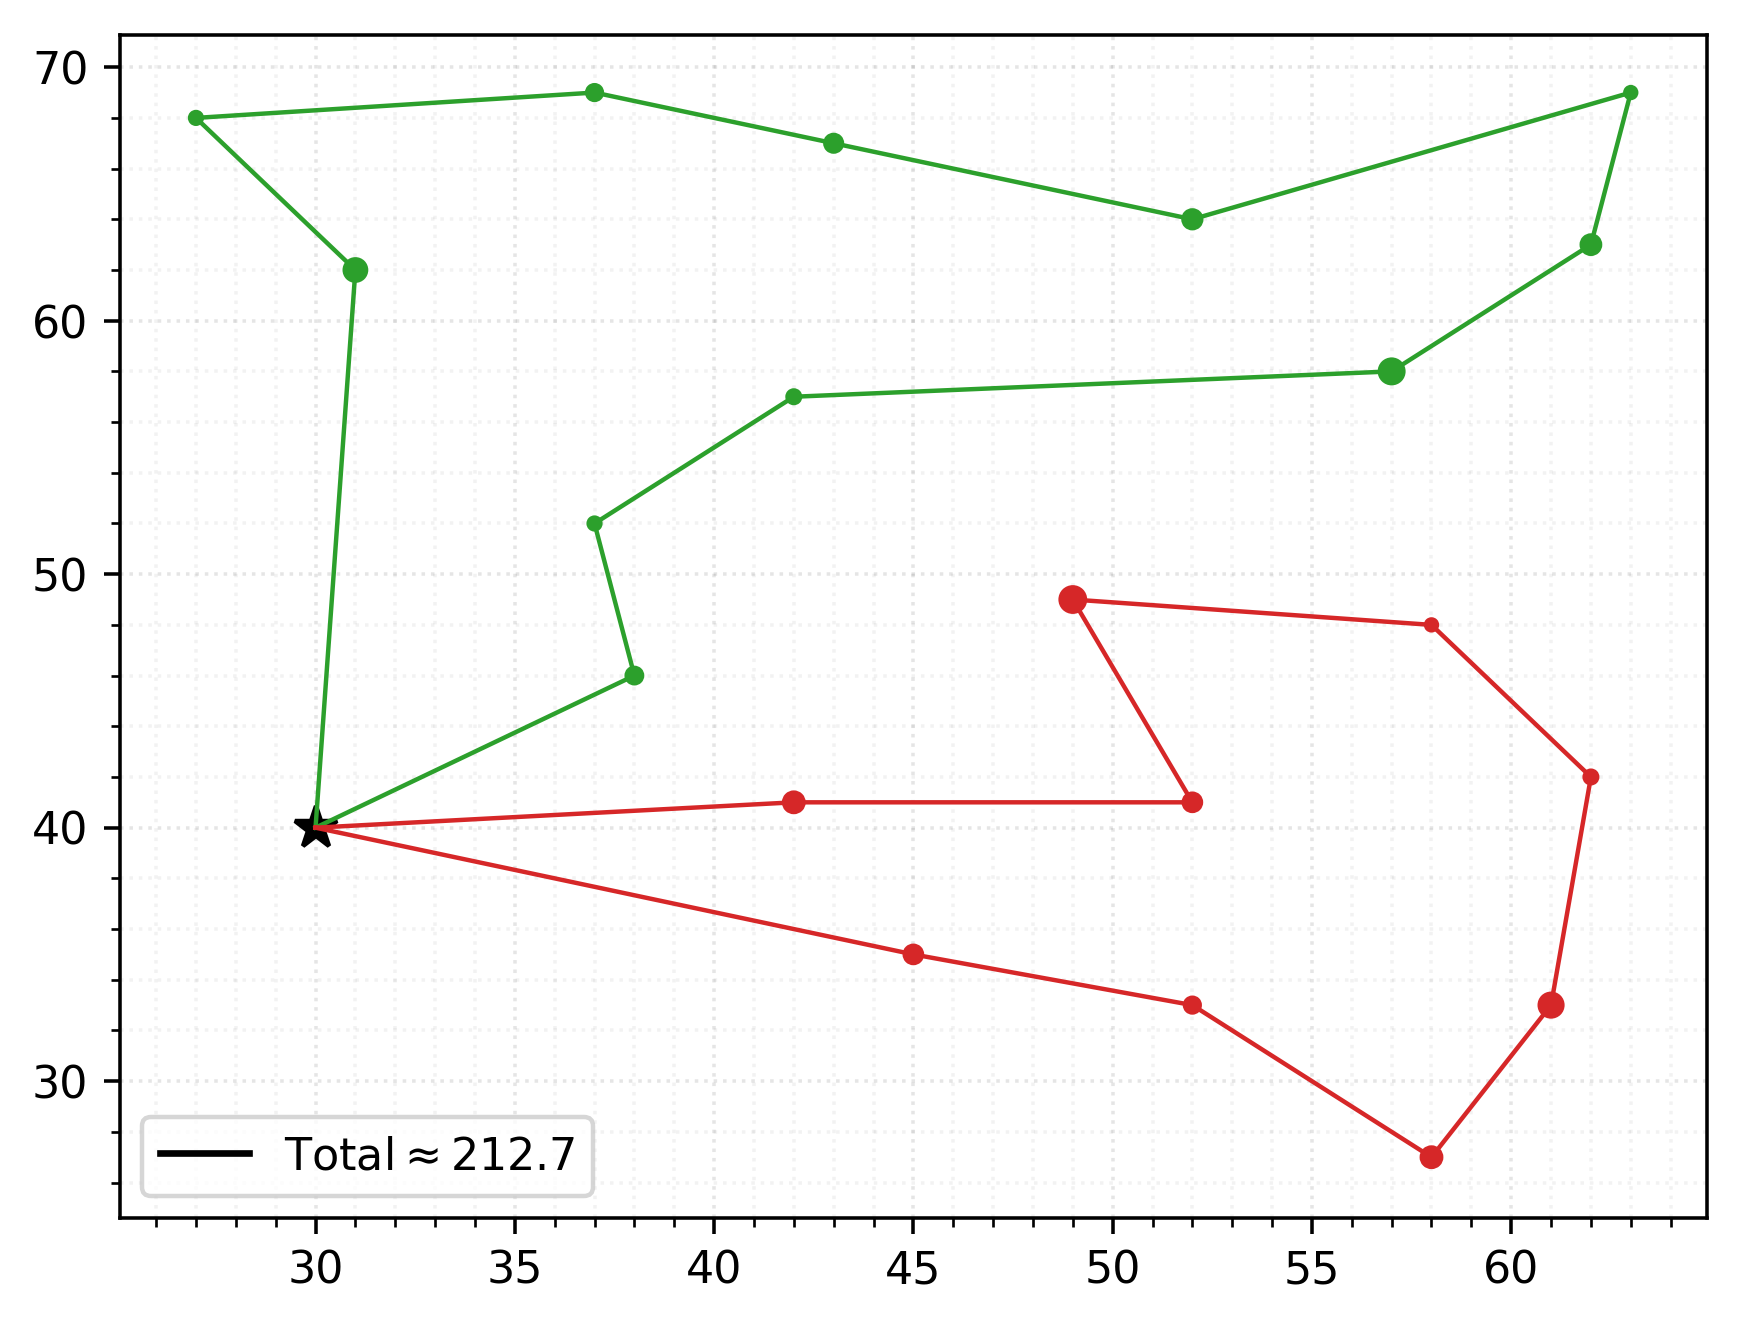
\includegraphics[width=1\textwidth]{images/savings/optimochico}
		\caption{\footnotesize Ruta óptima para la instancia \textbf{P-n21-k2}}
		\label{fig:savings-optimo-chico}
	\end{minipage}%
\end{figure}
Si bien las soluciones óptimas tienen una forma de ruta distinta entre sí, podemos notar que saving en ambos casos dio esta forma de ruta. 
\par Otro caso que pertenecerá al mismo data set que los últimos dos, con los que experimentaremos luego es el de la figura \ref{fig:savings-malo-grande}. Aquí es más marcada la diferencia entre ambos recorridos, siendo savings un 15.2\% peor que la óptima.
\begin{figure}[H]
	\centering
	\begin{minipage}{0.35\textwidth}
		\centering
		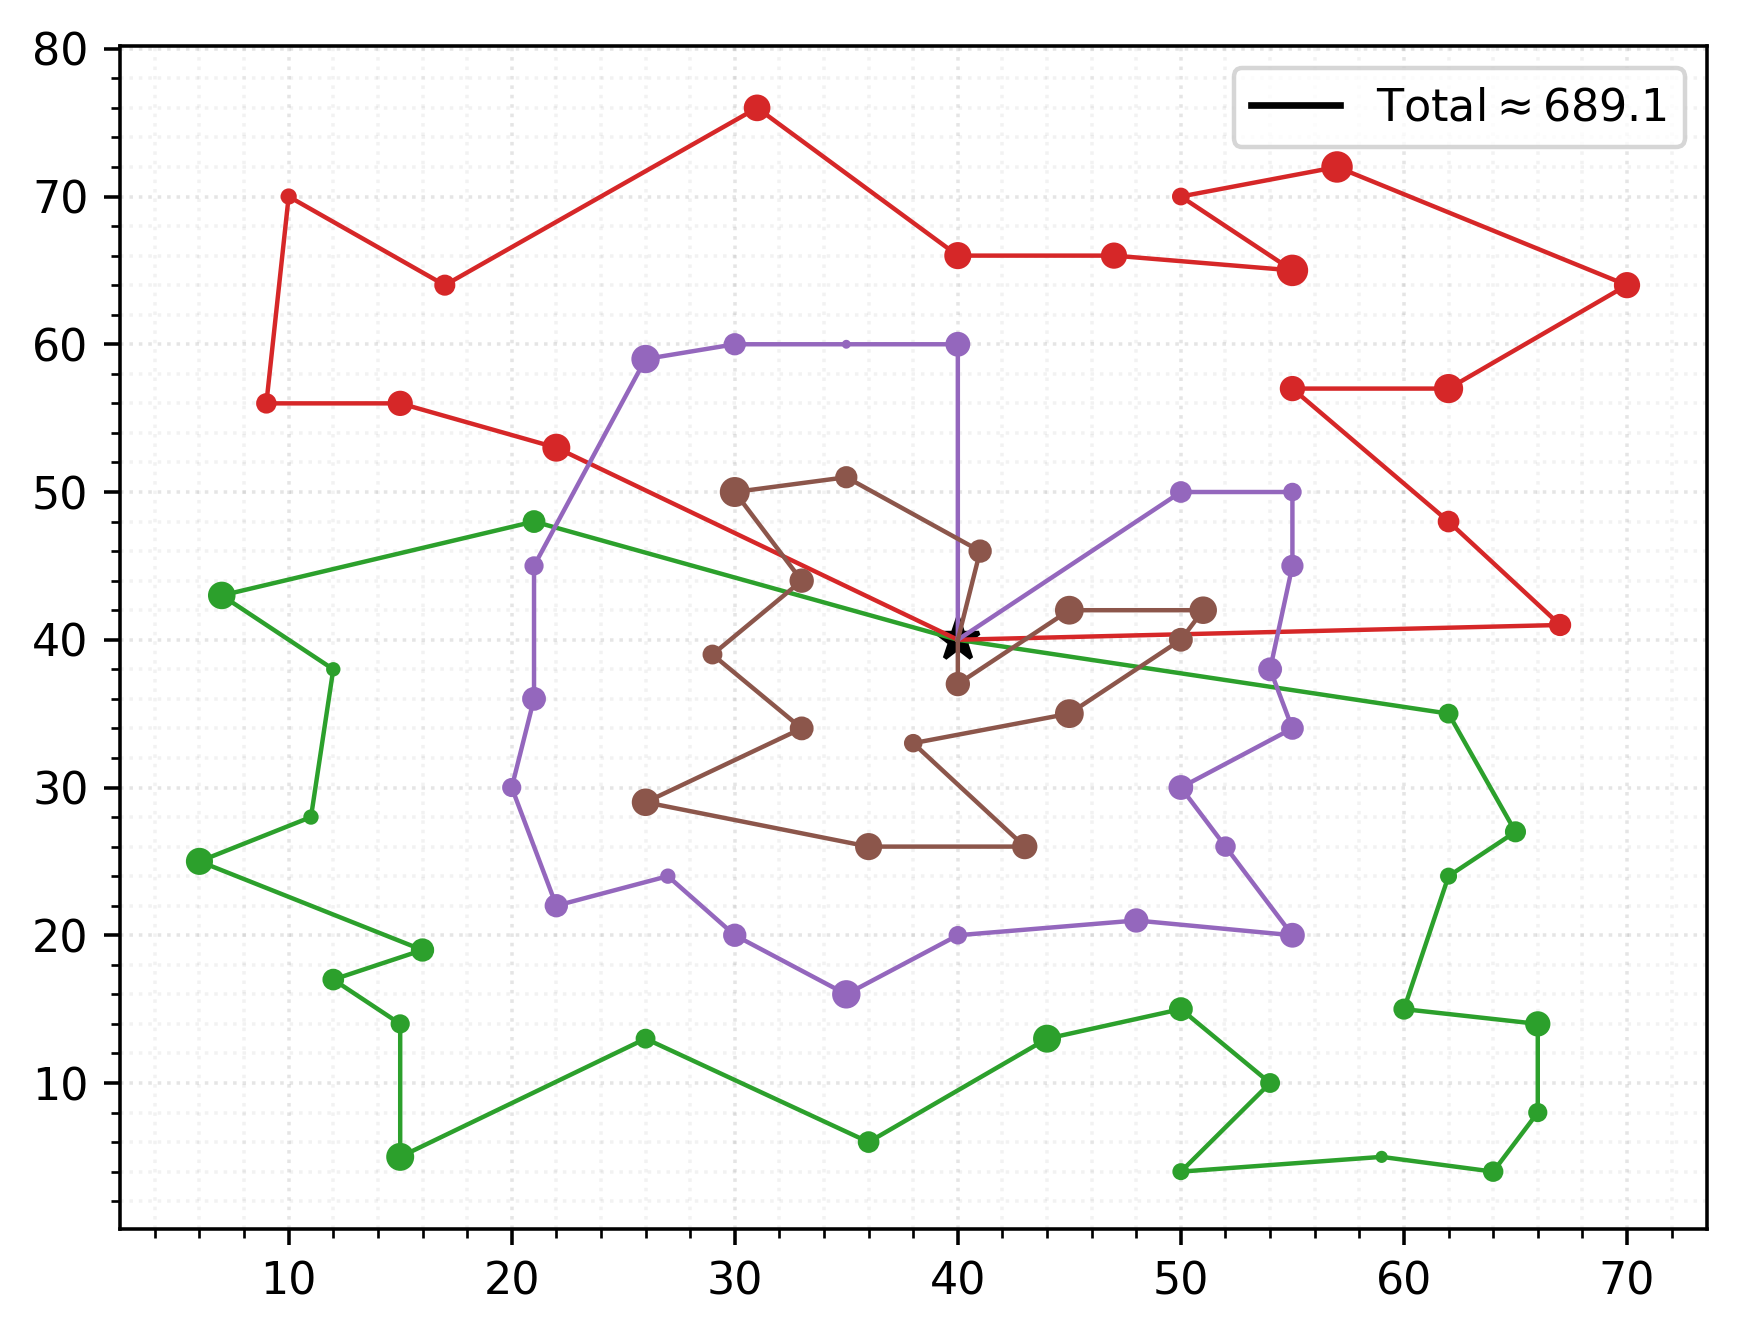
\includegraphics[width=1\textwidth]{images/savings/malosavinggrande}
		\caption{\footnotesize Ruta resultado savings para la instancia \textbf{P-n76-k4}}
		\label{fig:savings-malo-grande}
	\end{minipage}%
	\hspace{0.03\textwidth}
	\begin{minipage}{0.35\textwidth}
		\centering
		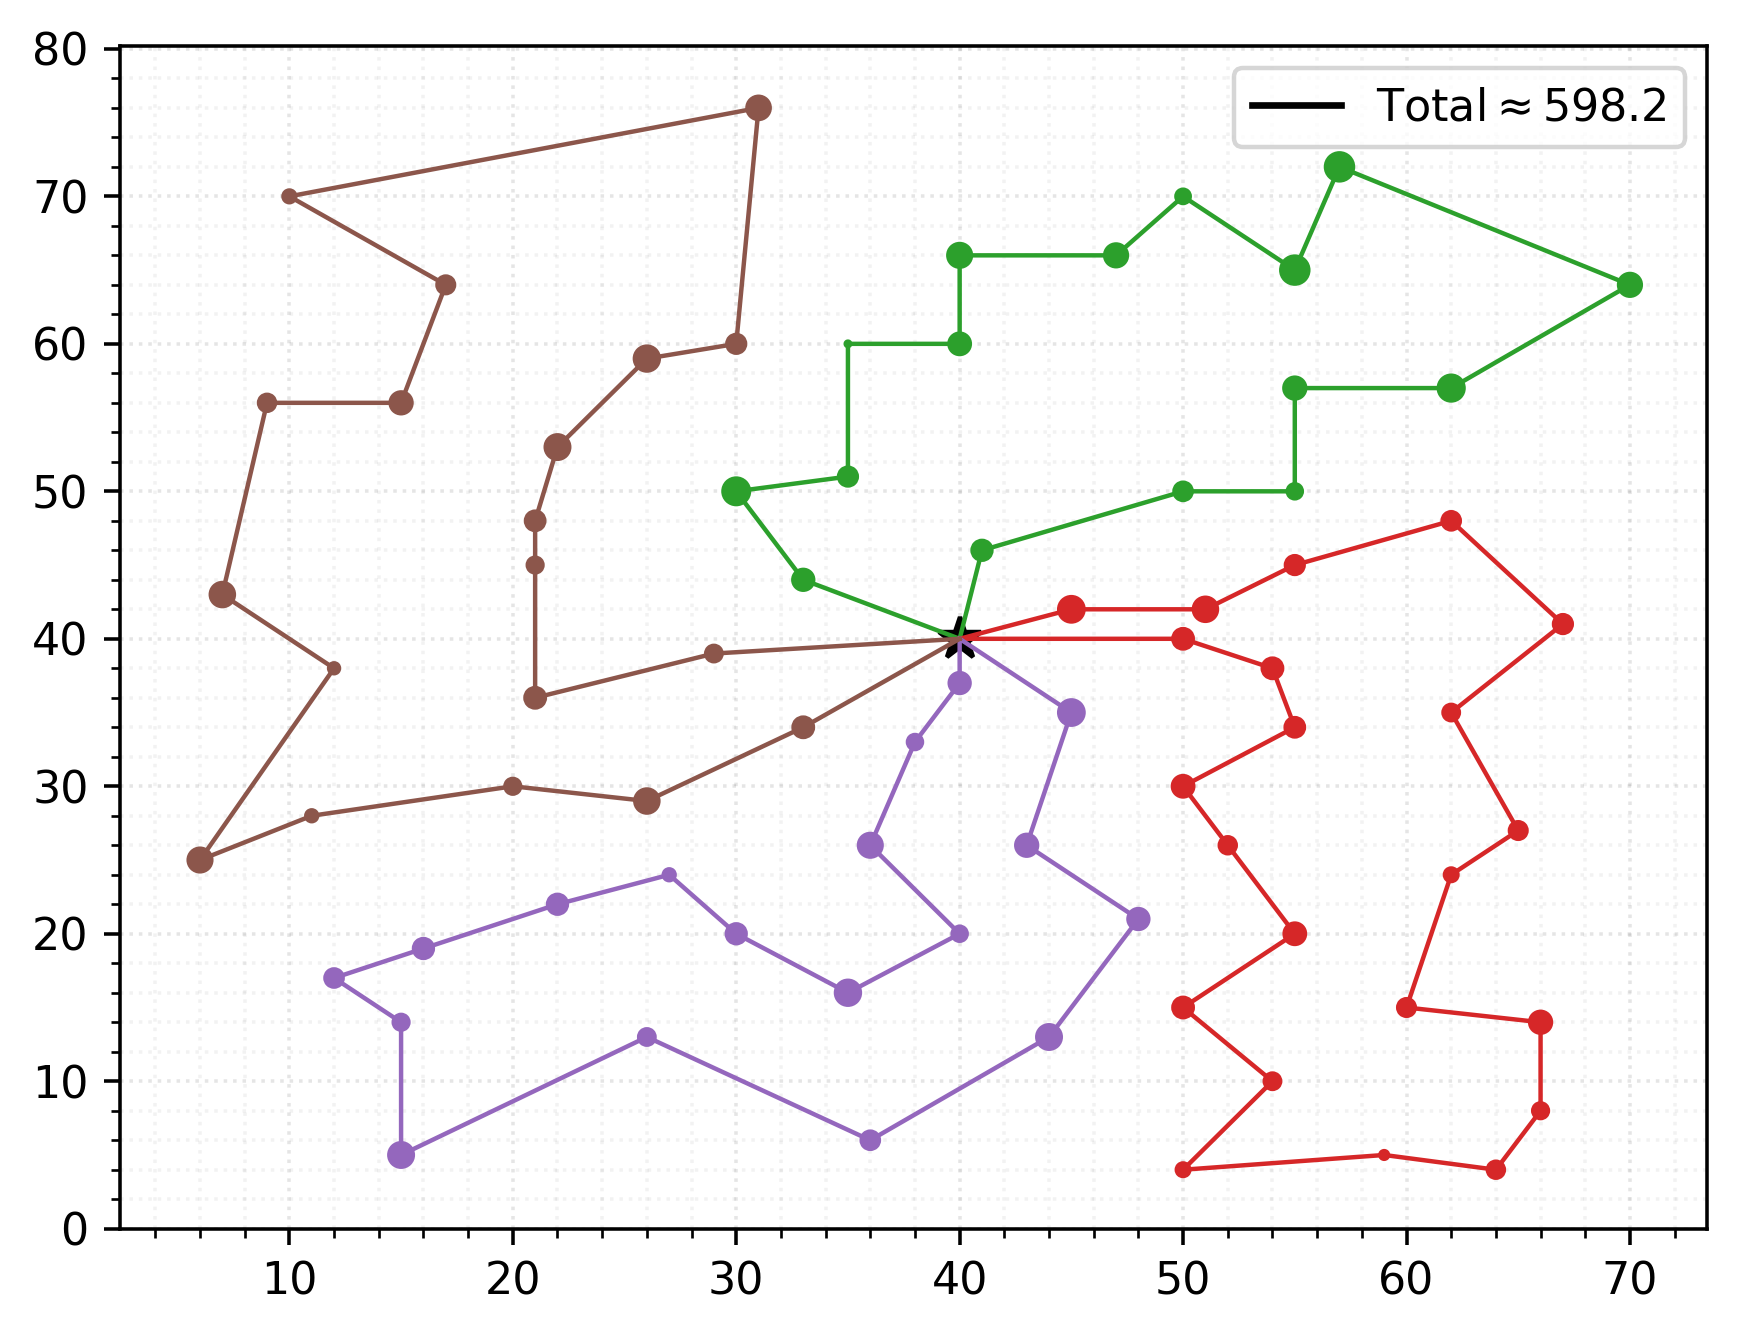
\includegraphics[width=1\textwidth]{images/savings/optimogrande}
		\caption{\footnotesize Ruta óptima para la instancia \textbf{P-n76-k4}}
		\label{fig:savings-optimo-grande}
	\end{minipage}%
\end{figure}

